%!TEX program = xelatex
\documentclass[UTF8,zihao=5]{ctexart} %ctex包的article


\usepackage[hidelinks]{hyperref}%超链接,自动加到目录里面



\title{{\bfseries\rmfamily\Huge{高等计算流体力学\hspace{1em}\\第6次作业}}}
\author{周涵宇 2022310984}
\date{}

\usepackage[a4paper]{geometry}
\geometry{left=0.75in,right=0.75in,top=1in,bottom=1in}%纸张大小和页边距

\usepackage[
UseMSWordMultipleLineSpacing,
MSWordLineSpacingMultiple=1.5
]{zhlineskip}%office风格的行间距

\usepackage{fontspec}
\setmainfont{Times New Roman}
\setsansfont{Source Sans Pro}
\setmonofont{Latin Modern Mono}
\setCJKmainfont{SimSun}[AutoFakeBold=true]
% \setCJKmainfont{仿宋}[AutoFakeBold=true]
\setCJKsansfont{黑体}[AutoFakeBold=true]
\setCJKmonofont{DengXian}[AutoFakeBold=true]

\setCJKfamilyfont{kaiti}{楷体}
\newfontfamily\CM{Cambria Math}


% \usepackage{indentfirst} %不工作 怎样调整ctex的段首缩进大小呢

\usepackage{fancyhdr}
\pagestyle{fancy}
\lhead{}
\chead{}
\rhead{}
\lfoot{}
\cfoot{\thepage}
\rfoot{}
\renewcommand{\headrulewidth}{1pt} %改为0pt即可去掉页眉下面的横线
\renewcommand{\footrulewidth}{1pt} %改为0pt即可去掉页脚上面的横线
\setcounter{page}{1}


% \usepackage{bm}

\usepackage{amsmath,amsfonts}
\usepackage{array}
\usepackage{enumitem}
\usepackage{unicode-math}

% \usepackage{titlesec} % it subverts the ctex titles
\usepackage{titletoc}


% titles in toc:
\titlecontents{section}
              [2cm]
              {\sffamily\zihao{5}\mdseries}%
              {\contentslabel{3em}}%
              {}%
              {\titlerule*[0.5pc]{-}\contentspage\hspace*{1cm}}

\titlecontents{subsection}
              [3cm]
              {\rmfamily\mdseries\zihao{5}}%
              {\contentslabel{3em}}%
              {}%
              {\titlerule*[0.5pc]{-}\contentspage\hspace*{1cm}}

\titlecontents{subsubsection}
              [4cm]
              {\rmfamily\mdseries\zihao{5}}%
              {\contentslabel{3em}}%
              {}%
              {\titlerule*[0.5pc]{-}\contentspage\hspace*{1cm}}
\renewcommand*\contentsname{\hfill \sffamily\mdseries 目录 \hfill}

\ctexset{
    section={   
        % name={前面,后面},
        number={\arabic{section}.},
        format=\sffamily\raggedright\zihao{4}\mdseries,
        indent= {0em},
        aftername = \hspace{0.5em},
        beforeskip=1ex,
        afterskip=1ex
    },
    subsection={   
        % name={另一个前面,另一个后面},
        number={\arabic{section}.\arabic{subsection}.}, %如果只用一个数字而非1.1
        format=\rmfamily\raggedright\mdseries\zihao{5},%正体字体,不加粗,main字体,五号字
        indent = {2em}, %缩进
        aftername = \hspace{0.5em},
        beforeskip=1ex,
        afterskip=1ex
    },
    subsubsection={   
        % name={另一个前面,另一个后面},
        number={\arabic{section}.\arabic{subsection}.\arabic{subsubsection}.}, %默认的 1.1.1
        format=\rmfamily\raggedright\mdseries\zihao{5},%无衬线字体,加粗,sans字体,五号字
        indent = {2em}, %缩进
        aftername = \hspace{0.5em},  %名字和标题间插入字符(此处是空白)
        beforeskip=1ex, %空行
        afterskip=1ex
    }
}

\usepackage{float}
\usepackage{graphicx}
\usepackage{multirow}
\usepackage{multicol}
\usepackage{caption}
\usepackage{subcaption}
\usepackage{cite}


%part、section、subsection、subsubsection、paragraph、subparagraph
\newcommand{\bm}[1]{{\mathbf{#1}}}
\newcommand{\trans}[0]{^\mathrm{T}}
\newcommand{\tran}[1]{#1^\mathrm{T}}
\newcommand{\hermi}[0]{^\mathrm{H}}
\newcommand{\conj}[1]{\overline{#1}}
\newcommand*{\av}[1]{\left\langle{#1}\right\rangle}
\newcommand*{\avld}[1]{\frac{\overline{D}#1}{Dt}}
\newcommand*{\pd}[2]{\frac{\partial #1}{\partial #2}}
\newcommand*{\pdcd}[3]{\frac{\partial^2 #1}{\partial #2 \partial #3}}
\newcommand*{\inc}[0]{{\Delta}}

\newcommand*{\uu}[0]{\bm{u}}
\newcommand*{\vv}[0]{\bm{v}}
\newcommand*{\g}[0]{\bm{g}}
\newcommand*{\nb}[0]{{\nabla}}



\begin{document}

\maketitle

\section{迎风型有限差分方法解欧拉方程}

求解双曲守恒律方程:
\begin{equation}
    \pd{U}{t}+\pd{F}{x}+\pd{G}{y}=0
\end{equation}

其中每个方向采用守恒型离散:
$$
    \left[\pd{F}{x}\right]_i =
    \frac{F_{i+1/2}-F_{i-1/2}}{\inc x}
$$
对于每个$i+1/2$半节点值,可用$i,i+1$上的中心插值分别给出
$F_{i+1/2,-},F_{i+1/2,+},U_{i+1/2,-},U_{i+1/2,+}$,随后采用迎风型方法计算半节点值。假如采用Roe格式,则为:
$$
    F_{f}=\tilde{L}_f\frac{I+sign(\tilde{\Lambda}_f)}{2}\tilde{R}_fF_{f,-}+\tilde{L}_f\frac{I-sign(\tilde{\Lambda}_f)}{2}\tilde{R}_fF_{f,+}
$$
其中$f$是指的$i+1/2$等半节点指标。
假如采用原始Lax格式,可考虑:
$$
    F_{f}=\frac{1}{2}(F_{f,-}+F_{f,+}-\max|\lambda_f|(U_{f,+}-U_{f,-}))
$$
本文方便起见,取Lax格式实现迎风性。

至此,只需要确定笛卡尔网格上的高阶插值过程计算半节点的$U,F$等。
考虑有限差分形式的,
原始的WENO5格式\cite{jiang1996efficient},
以及文献\cite{henrick2005mapped}中给出的WENO5m格式。
其中,根据Jiang,Shu等的方案\cite{jiang1996efficient},不同子模板的非线性权为:
$$
    \omega_k=\frac{\bar\omega_k}{(\epsilon+\beta_k)^{p}}
$$
其中$\bar\omega_k$是理想(线性)权,
$\beta_k$是子模版的间断探测器,与\cite{jiang1996efficient}相同。
根据阶数要求和推荐,取$p=2$。
$\epsilon$取较小时,对间断的限制较强;
$\epsilon\rightarrow\infty$时,退化为线性的五阶迎风(UW5)格式。

光滑解上原始的WENO5有较大误差,Henrick等给出简单的非线性权重映射方式提升光滑解的精度\cite{henrick2005mapped}。

本文计算域都是笛卡尔积,因此不作参数映射。

以上给出了空间离散,整理为半离散格式
$$
    \frac{d}{dt}U_i^n=R(U_i^{n+1})
$$
方便起见采用经典显式四级四阶RK方法时间推进。Butcher表为:
\begin{table}[H]
    \footnotesize
    \begin{center}
        \caption{RK4 Butcher表} %需要学习统一设置;0代表不变?
        \begin{tabular}{c|cccc}
            $0$                                                                           \\
            $\frac{1}{2}$ & $\frac{1}{2}$                                                 \\
            $\frac{1}{2}$ & $0$           & $\frac{1}{2}$                                 \\
            $1$           & $0$           & $0$           & $1$                           \\
            \hline
                          & $\frac{1}{6}$ & $\frac{1}{3}$ & $\frac{1}{3}$ & $\frac{1}{6}$
        \end{tabular}
    \end{center}
\end{table}

以上离散方法的理论精度阶数为4,由时间推进限制。

\subsection{线性对流方程间断解}

首先验证WENO格式对间断的振荡抑制能力。取线性对流方程,即
$$
    U=u,\ F=a_x u,\ G=a_y u
$$
其中对流速度取$a_x=a_y=1$,CFL数取$0.5$,计算域$[0,1]\times[0,1]$周期边界,计算1的时间长度为一个周期。
初值为$u=0.5-0.5sign((x-0.5)^2+(y-0.5^2)-0.25^2)$,即一个圆形凸台。
取$64\times64$网格:$t=1$的结果如下:
\begin{figure}[H]
    \begin{minipage}[c]{0.32\linewidth}  %需调整
        \centering
        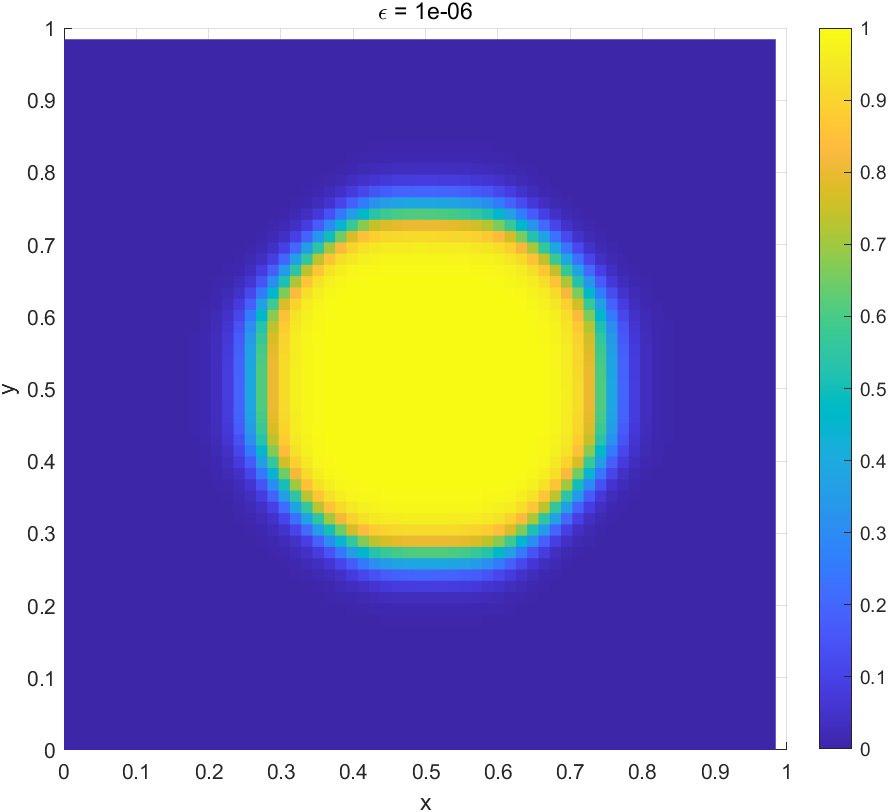
\includegraphics[width=5cm]{Linconv_E6.png}  %需调整
    \end{minipage}
    \hfill %弹性长度
    \begin{minipage}[c]{0.32\linewidth}  %需调整
        \centering
        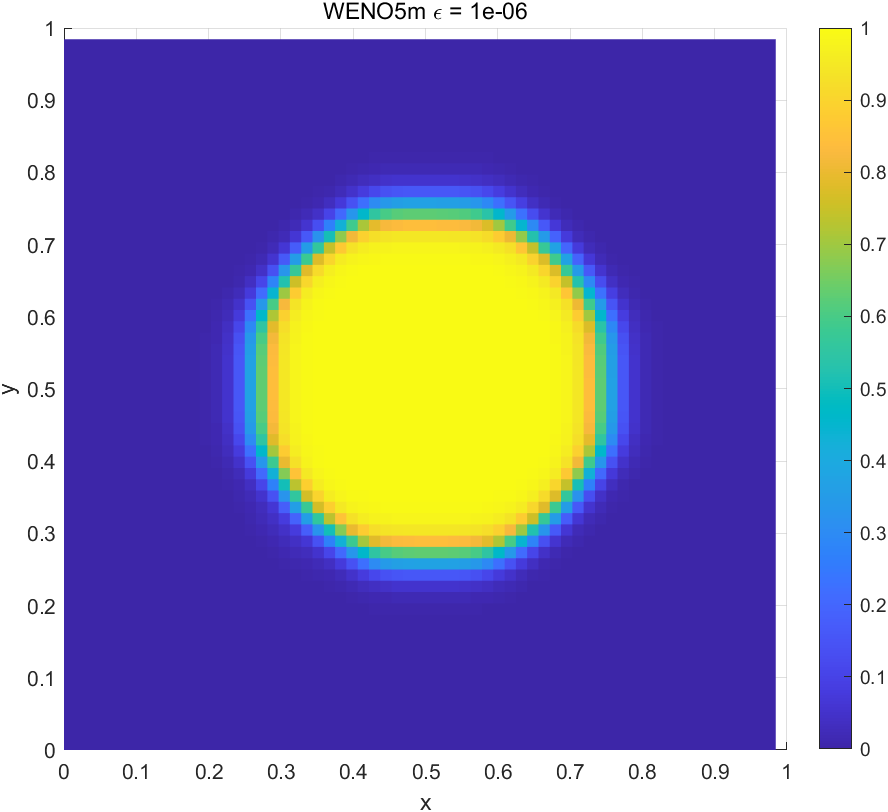
\includegraphics[width=5cm]{Linconv_E6m.png}  %需调整
    \end{minipage}
    \hfill %弹性长度
    \begin{minipage}[c]{0.32\linewidth}  %需调整
        \centering
        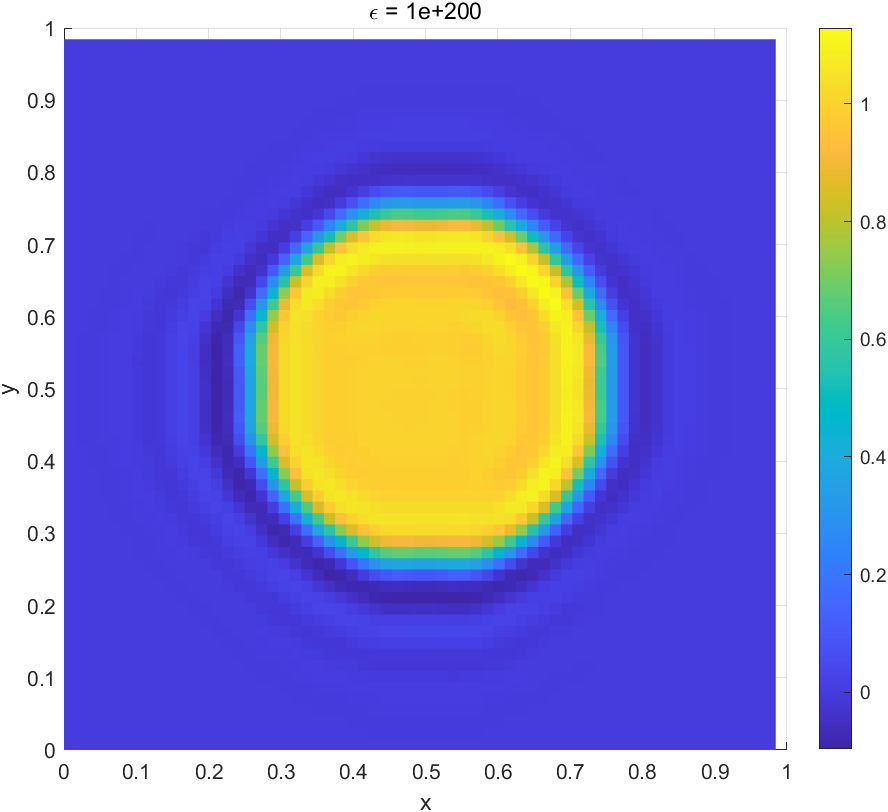
\includegraphics[width=5cm]{Linconv_LIN.png}  %需调整
    \end{minipage}
    \caption{线性对流,WENO5 WENO5m UW5, 其中取$\epsilon=10^{-6}$}
\end{figure}
可见线性格式有明显振荡而WENO5和WENO5m都成功抑制了振荡,$\epsilon=1e-6$时解保持了单调性。

\subsection{等熵涡算例}

计算量热理想气体二维Euler方程。
考虑等熵涡问题,具体问题设置与\cite{hu1999weighted}都一样,
涡强度$\chi=5$,位置在$(5,5)$,计算域$[0,10]\times[0,10]$,
取周期边界。时间步长取$h_x$,相当于约为$0.2$的CFL数。

由于计算域是周期的而非无限大,实际上初始位置边界上有一个极小的间断,
速度间断可达$10^{-7}$级别。为了避免这个解析解中不存在的间断的影响,
考虑欧拉方程的信息传播,在$t=2$时,$[5,9]\times[5,9]$中的解都没有
受到边界的影响,因此考虑$t=2$的误差对比时,取范数:
$$
    \|\rho-\rho_{ana}\|_{L1} =
    \inc x\inc y\sum_{(x_i,y_j)\in[5,9]\times[5,9]}{|\rho(x_i,y_j)-\rho(x_i,y_j)_{ana}|}
$$

下表给出了不同格式的计算误差和收敛阶数。

\begin{table}[H]
    \footnotesize
    \begin{center}
        \caption{等熵涡误差$\|\rho-\rho_{ana}\|_{L1}, t=2$} %需要学习统一设置;0代表不变?
        \begin{tabular}{|c|c|c|c|c|c|c|c|c|}
            \hline
            \multirow{2}{*}{$h$} & \multicolumn{2}{|c|}{WENO5 $\epsilon=10^{-6}$} & \multicolumn{2}{|c|}{WENO5 $\epsilon=10^{-3}$} & \multicolumn{2}{|c|}{WENO5m $\epsilon=10^{-6}$} & \multicolumn{2}{|c|}{UW5}                                                                             \\
            \cline{2-9}
                                 & $\|\rho-\rho_{ana}\|_{L1}$                     & 阶数                                           & $\|\rho-\rho_{ana}\|_{L1}$                      & 阶数                      & $\|\rho-\rho_{ana}\|_{L1}$ & 阶数   & $\|\rho-\rho_{ana}\|_{L1}$ & 阶数   \\
            \hline
            $1/20$               & 3.1230530e-01                                  &                                                & 2.9349690e-01                                   &                           & 2.2693522e-01              &        & 9.5435399e-02              &        \\
            \hline
            $1/40$               & 5.2543401e-02                                  & 2.5714                                         & 3.2229027e-02                                   & 3.1869                    & 2.9438651e-02              & 2.9465 & 1.2498203e-02              & 2.9328 \\
            \hline
            $1/80$               & 4.4590657e-03                                  & 3.5587                                         & 2.4662220e-03                                   & 3.7080                    & 9.2472577e-04              & 4.9925 & 6.0787613e-04              & 4.3618 \\
            \hline
            $1/160$              & 2.5012196e-04                                  & 4.1560                                         & 8.1062336e-05                                   & 4.9271                    & 2.2989118e-05              & 5.3300 & 2.0860055e-05              & 4.8650 \\
            \hline
            $1/320$              & 1.1233154e-05                                  & 4.4768                                         & 1.9013022e-06                                   & 5.4140                    & 6.6682832e-07              & 5.1075 & 6.6494326e-07              & 4.9714 \\
            \hline
            $1/640$              & 3.7072570e-07                                  & 4.9213                                         & 4.4152115e-08                                   & 5.4284                    & 2.0893558e-08              & 4.9962 & 2.0892949e-08              & 4.9921 \\
            \hline
        \end{tabular}
    \end{center}
\end{table}

同时,给出不同格式误差$\rho-\rho_{ana}$的空间分布:
\begin{figure}[H]
    \begin{minipage}[c]{0.32\linewidth}  %需调整
        \centering
        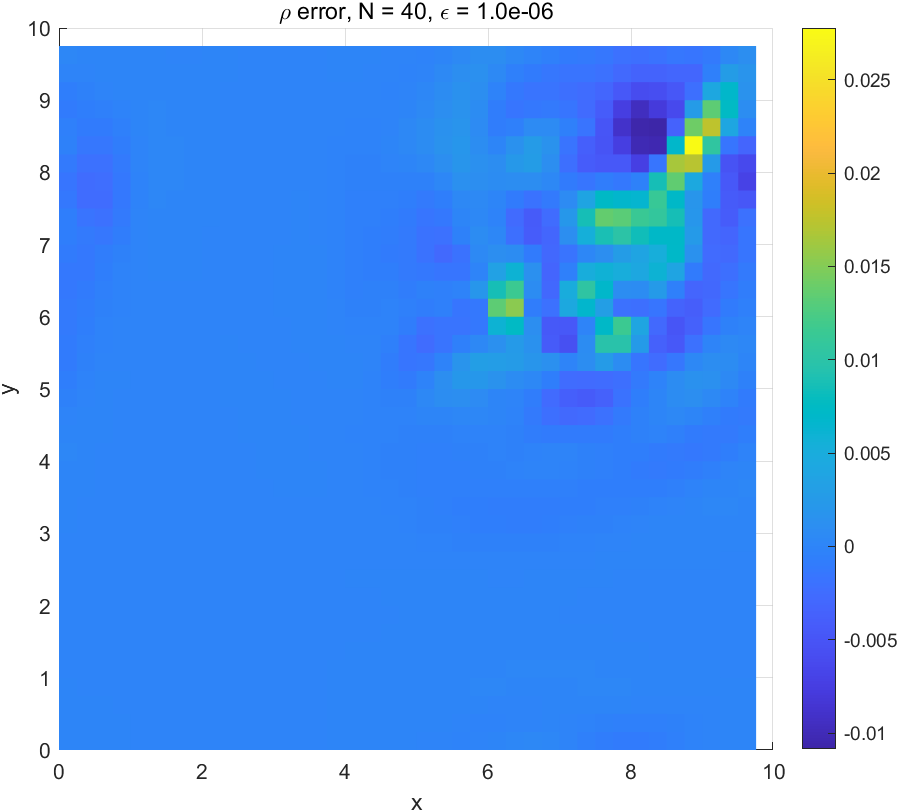
\includegraphics[width=5cm]{Err_40_E6.png}  %需调整
    \end{minipage}
    \hfill %弹性长度
    \begin{minipage}[c]{0.32\linewidth}  %需调整
        \centering
        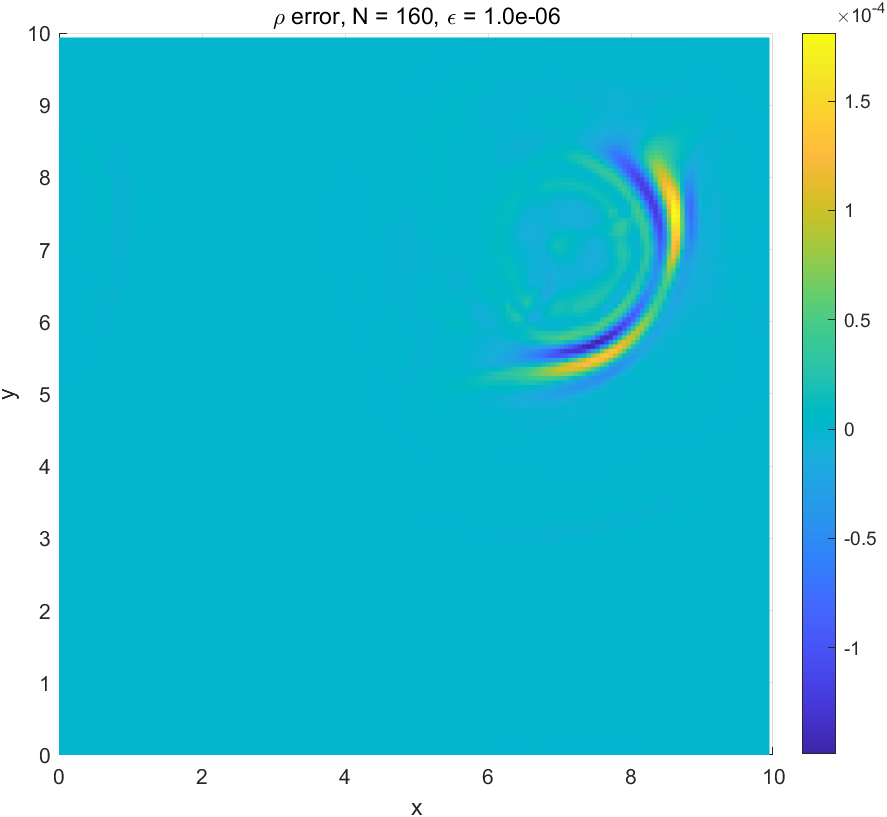
\includegraphics[width=5cm]{Err_160_E6.png}  %需调整
    \end{minipage}
    \hfill %弹性长度
    \begin{minipage}[c]{0.32\linewidth}  %需调整
        \centering
        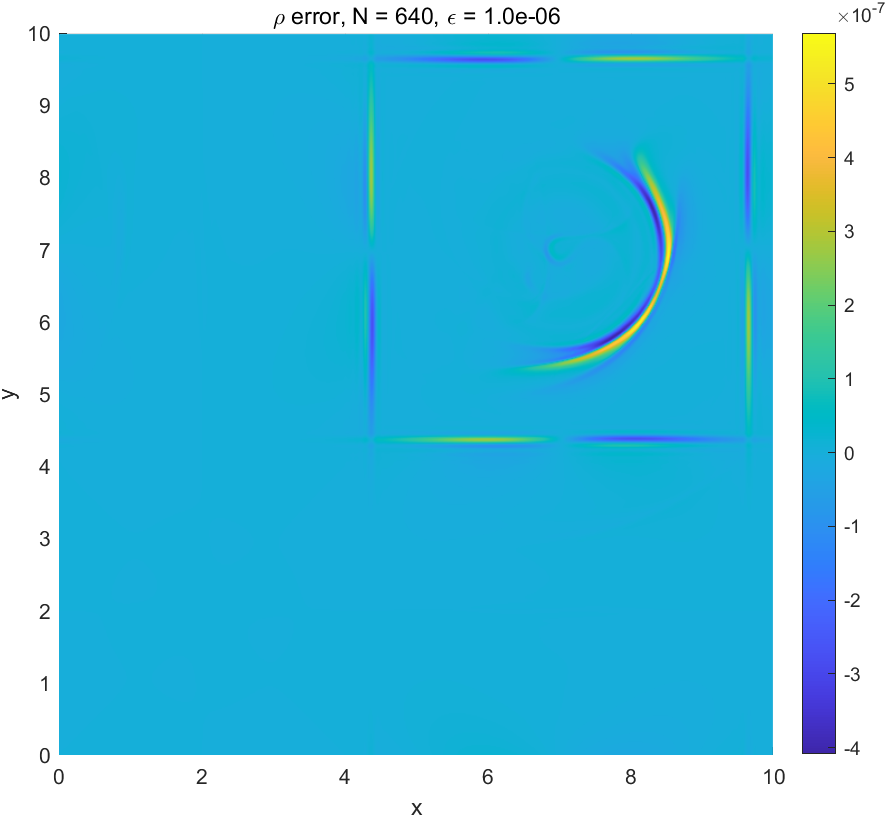
\includegraphics[width=5cm]{Err_640_E6.png}  %需调整
    \end{minipage}
    \caption{等熵涡$\rho-\rho_{ana}$,WENO5 $\epsilon=10^{-6}$,分别$h=1/40,1/160,1/640$}
\end{figure}

\begin{figure}[H]
    \begin{minipage}[c]{0.32\linewidth}  %需调整
        \centering
        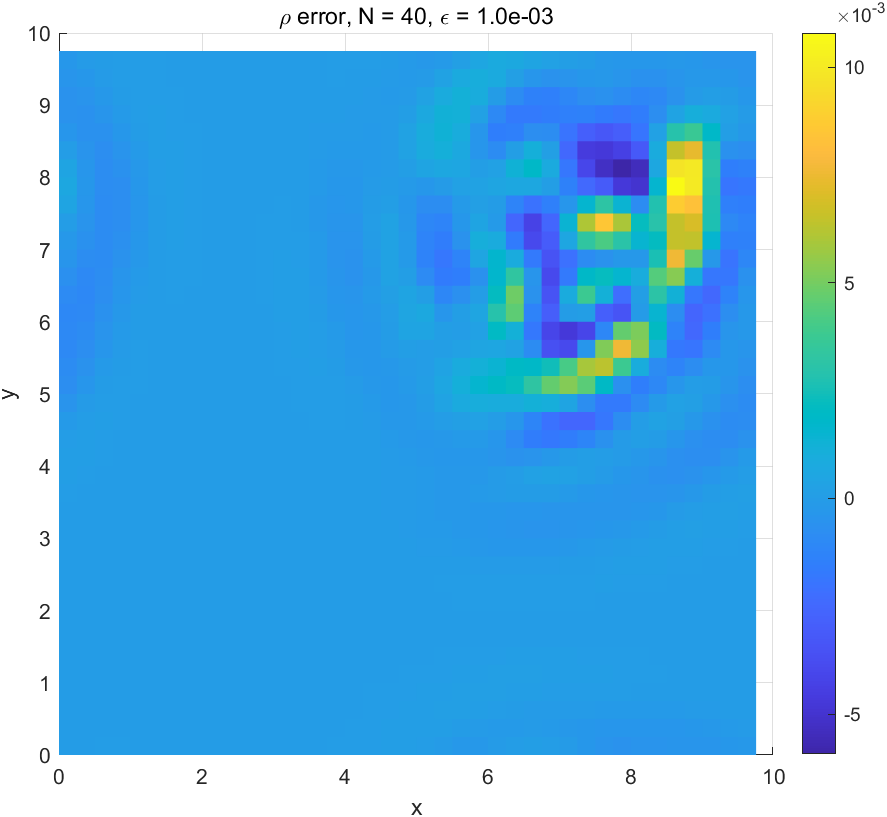
\includegraphics[width=5cm]{Err_40_E3.png}  %需调整
    \end{minipage}
    \hfill %弹性长度
    \begin{minipage}[c]{0.32\linewidth}  %需调整
        \centering
        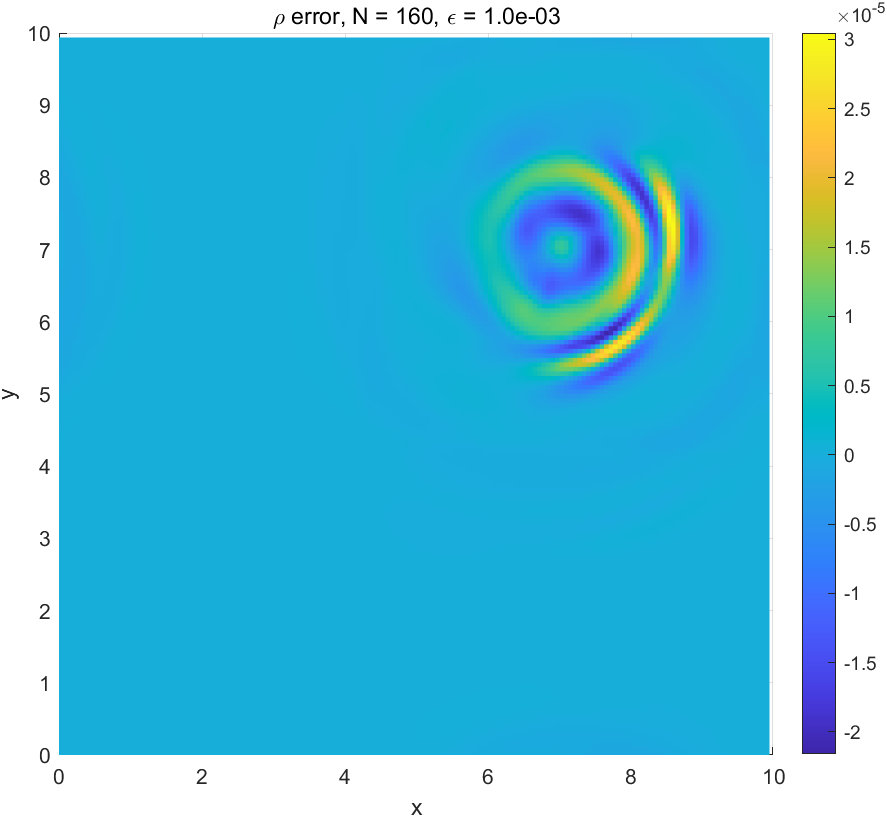
\includegraphics[width=5cm]{Err_160_E3.png}  %需调整
    \end{minipage}
    \hfill %弹性长度
    \begin{minipage}[c]{0.32\linewidth}  %需调整
        \centering
        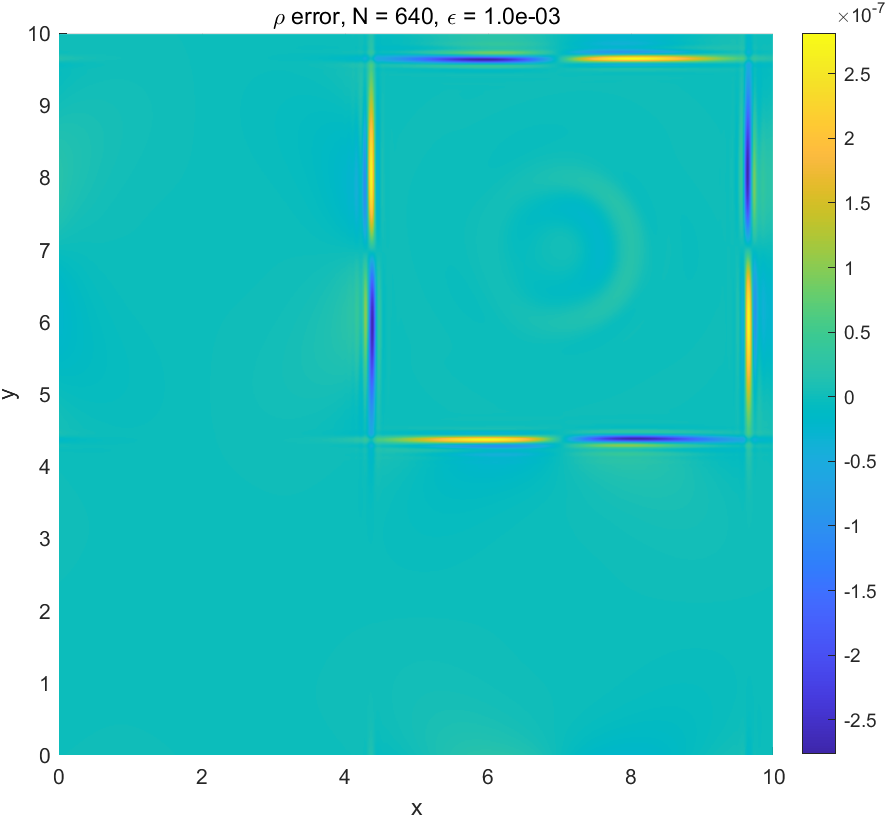
\includegraphics[width=5cm]{Err_640_E3.png}  %需调整
    \end{minipage}
    \caption{等熵涡$\rho-\rho_{ana}$,WENO5 $\epsilon=10^{-3}$,分别$h=1/40,1/160,1/640$}
\end{figure}

\begin{figure}[H]
    \begin{minipage}[c]{0.32\linewidth}  %需调整
        \centering
        \includegraphics[width=5cm]{Err_40_E6m.png}  %需调整
    \end{minipage}
    \hfill %弹性长度
    \begin{minipage}[c]{0.32\linewidth}  %需调整
        \centering
        \includegraphics[width=5cm]{Err_160_E6m.png}  %需调整
    \end{minipage}
    \hfill %弹性长度
    \begin{minipage}[c]{0.32\linewidth}  %需调整
        \centering
        \includegraphics[width=5cm]{Err_640_E6m.png}  %需调整
    \end{minipage}
    \caption{等熵涡$\rho-\rho_{ana}$,WENO5m $\epsilon=10^{-6}$,分别$h=1/40,1/160,1/640$}
\end{figure}

\begin{figure}[H]
    \begin{minipage}[c]{0.32\linewidth}  %需调整
        \centering
        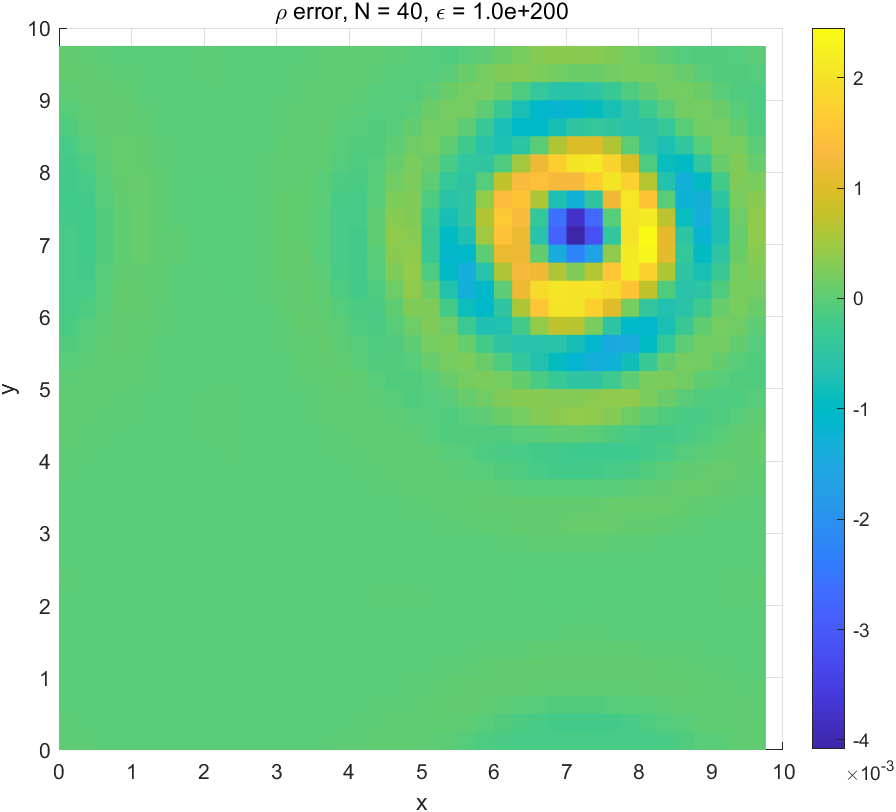
\includegraphics[width=5cm]{Err_40_LIN.png}  %需调整
    \end{minipage}
    \hfill %弹性长度
    \begin{minipage}[c]{0.32\linewidth}  %需调整
        \centering
        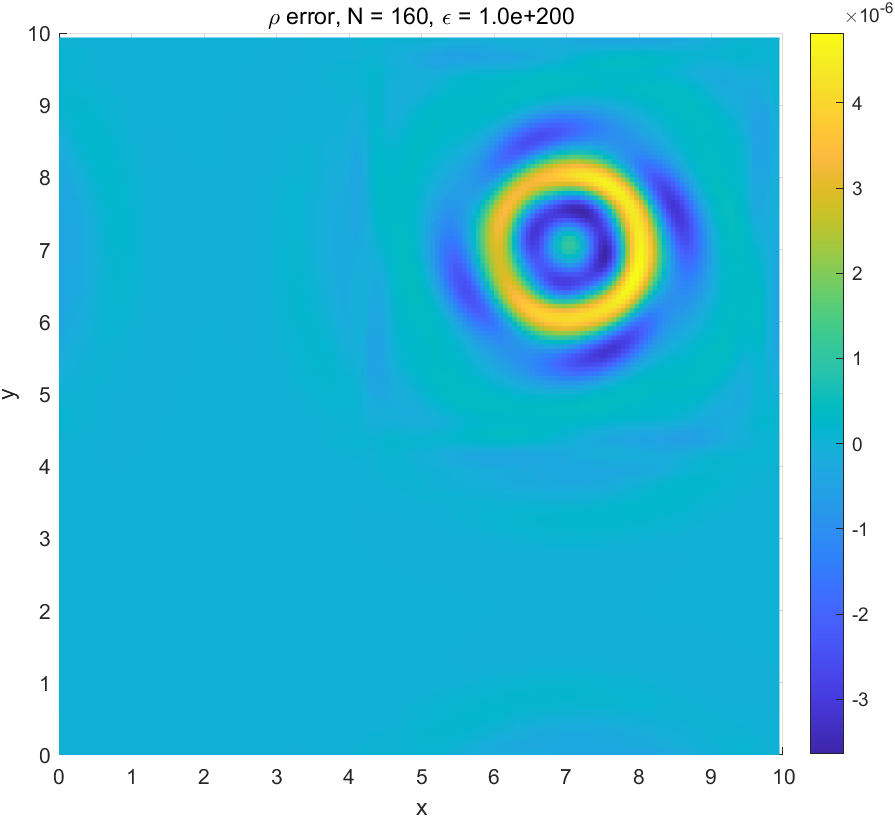
\includegraphics[width=5cm]{Err_160_LIN.png}  %需调整
    \end{minipage}
    \hfill %弹性长度
    \begin{minipage}[c]{0.32\linewidth}  %需调整
        \centering
        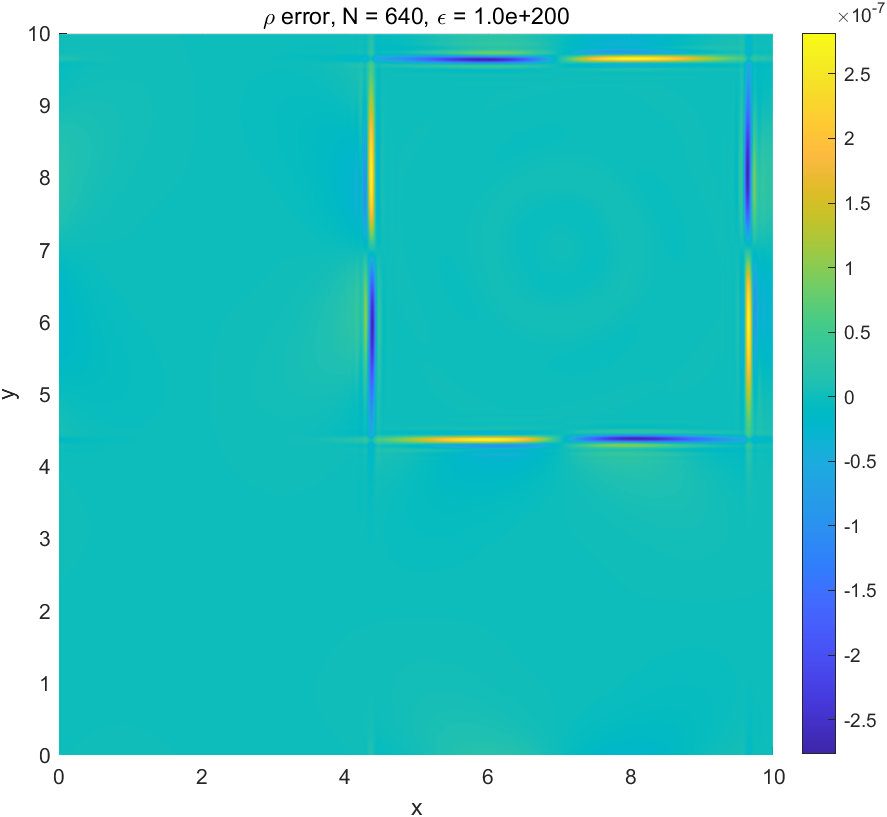
\includegraphics[width=5cm]{Err_640_LIN.png}  %需调整
    \end{minipage}
    \caption{等熵涡$\rho-\rho_{ana}$,UW5,分别$h=1/40,1/160,1/640$}
\end{figure}
首先可见所有$h=1/640$的网格上边界间断带来的误差已经成为主导,
同时所有算例中格式本身的误差都集中在非平凡区域$[5,9]\times[5,9]$中,
这意味着误差在空间范围的截取是合理且必要的。

接着,所有格式中线性格式的误差最小,WENO5m很接近线性格式。
而WENO5最差,同时增大$\epsilon$在牺牲间断单调性的情况下可减小一定误差。
因此可见,WENO5m可在有效抑制间断的同时,对光滑区计算误差很小。

线性迎风格式带来的误差更加各向同性,而所有非线性差分带来的误差有明显的非对称性和各向异性。

不同格式最高都可达到接近5阶的误差收敛,这超过了RK4的限制,而近乎达到了空间精度的阶数。


\bibliography{refs}{}
\bibliographystyle{unsrt}


\section*{附录}

本文使用的计算代码都在
\href{https://github.com/harryzhou2000/HW_ACFD}{Github的Git Repo(点击前往)}。























% \section{SECTION 节}

% 一个

% \subsection{SUBSECTION 小节}

% 示例

% \subsubsection{SUBSUBSECTION 小节节}

% 字体字号临时调整:
% {
%    \sffamily\bfseries\zihao{3} 哈哈哈哈哈 abcde %三号 sans系列字体(一开始设置的) 加粗
%    %只对大括号范围内的后面的字有用,在标题、题注里面同样
% }
% { 
%    \CJKfamily{kaiti}\zihao{5}\itshape 哈哈哈哈哈 abcde%三号 kaiti(一开始设置的, 斜体(英文有变)
%    %只对大括号范围内的后面的字有用,在标题、题注里面同样
% }

% 一大堆一大堆一大堆一大堆一大堆一大堆一大堆一大堆一大堆一大堆
% 一大堆一大堆一大堆一大堆一大堆一大堆一大堆一大堆一大堆一大堆一大堆一大堆
% 一大堆一大堆一大堆一大堆一大堆一大堆一大堆一大堆一大堆一大堆一大堆一大堆
% 一大堆一大堆一大堆一大堆一大堆一大堆一大堆一大堆一大堆一大堆一大堆一大堆

% \begin{center}
%     居中的什么乱七八糟东西
% \end{center}


% 一个列表:
% \begin{itemize}
%     \item asef
%     \item[\%] asdf
%     \item[\#] aaa
% \end{itemize}

% 一个有序列表:
% \begin{enumerate}
%     \item asef
%     \item[\%\%] asdf
%     \item aaa
% \end{enumerate}

% 一个嵌套列表,考虑缩进:
% \begin{enumerate}[itemindent=2em] %缩进
%     \item asef \par asaf 东西东西东西东西东西东西东西东西东西东西东西东西东西东西东西东西东西东西东西东西东西东西东西东西,
%           F不是不是不是不是不是不是不是不是不是不是不是不是不是不是不是
%           \begin{itemize}[itemindent=2em]  %缩进
%               \item lalala
%               \item mamama
%           \end{itemize}
%     \item asdf
%     \item aaa
% \end{enumerate}

% \section{SECTION}

% 图片排版:

% \begin{figure}[H]
%     \begin{minipage}[c]{0.45\linewidth}  %需调整
%         \centering
%         \includegraphics[width=8cm]{RAM_O2_4660.png}  %需调整
%         \caption{第一个图}
%         \label{fig:a}
%     \end{minipage}
%     \hfill %弹性长度
%     \begin{minipage}[c]{0.45\linewidth}  %需调整
%         \centering
%         \includegraphics[width=8cm]{RAM_O4_4660.png}  %需调整
%         \caption{第二个图}
%         \label{fig:b}
%     \end{minipage}
% \end{figure}

% figure的选项为“htbp”时,会自动浮动,是“H”则和文字顺序严格一些。

% \begin{figure}[H]
%     \begin{minipage}[c]{0.45\linewidth}  %需调整
%         \centering
%         \includegraphics[width=8cm]{RAM_O2_4660.png}  %需调整
%         \label{fig:x}
%     \end{minipage}
%     \hfill %弹性长度
%     \begin{minipage}[c]{0.45\linewidth}  %需调整
%         \centering
%         \includegraphics[width=8cm]{RAM_O4_4660.png}  %需调整
%         \label{fig:y}
%     \end{minipage}
%     \caption{第三个图}
% \end{figure}

% \begin{figure}[H]
%     \centering
%     \includegraphics[width=8cm]{RAM_O4_4660.png}  %需调整
%     \label{fig:c}
%     \caption{第四个图}
% \end{figure}



% \subsection{SUBSECTION}

% 关于怎么搞表格:

% \begin{table*}[htbp]
%     \footnotesize
%     \begin{center}
%         \caption{一端力矩载荷下的结果\fontsize{0pt}{2em}} %需要学习统一设置;0代表不变?
%         \label{表2}
%         \begin{tabular}{|c|c|c|c|c|c|c|}
%             \hline
%             节点数                              & 积分方案              & 单元数                & $h=1m$                & $h=0.1m$              & $h=0.05m$             & $h=0.01m$             \\
%             \hline
%             \multirow{6}{*}{2}                  & \multirow{3}{*}{精确} & 1                     & 4.235294117647059E-08 & 1.406250000000000E-06 & 2.862823061630218E-06 & 1.439654482924097E-05 \\
%             \cline{3-7}
%                                                 &                       & 10                    & 5.975103734439814E-08 & 4.235294117646719E-05 & 1.800000000000410E-04 & 1.406249999999849E-03 \\
%             \cline{3-7}
%                                                 &                       &
%             10000                               & 5.999999915514277E-08 & 5.999996622448291E-05 & 4.799989509752562E-04 & 5.999793702477535E-02                                                 \\
%             \cline{2-7}
%                                                 & \multirow{3}{*}{减缩} & 1                     & 6.000000000000001E-08 & 5.999999999999972E-05 & 4.799999999999911E-04 & 6.000000000003492E-02 \\
%             \cline{3-7}
%                                                 &                       & 10                    & 6.000000000000071E-08 & 5.999999999999142E-05 & 4.799999999995399E-04 & 5.999999999903294E-02 \\
%             \cline{3-7}
%                                                 &                       & 10000                 & 6.000000112649221E-08 & 5.999999234537814E-05 & 4.799997501925065E-04 & 6.000037607984510E-02 \\
%             \hline

%             \multirow{6}{*}{3}                  & \multirow{3}{*}{精确} & 1                     & 6.000000000000003E-08 & 6.000000000000202E-05 & 4.800000000000831E-04 & 6.000000000056749E-02 \\
%             \cline{3-7}
%                                                 &                       & 10                    & 5.999999999999932E-08 & 6.000000000004190E-05 & 4.800000000000206E-04 & 6.000000001613761E-02 \\
%             \cline{3-7}
%                                                 &                       & 10000                 & 6.000000013769874E-08 & 5.999989495410481E-05 & 4.799942099727246E-04 & 6.000263852944890E-02 \\
%             \cline{2-7}
%                                                 & \multirow{3}{*}{减缩} & 1                     & 6.000000000000002E-08 & 6.000000000000267E-05 & 4.800000000000754E-04 & 5.999999999989982E-02 \\
%             \cline{3-7}
%                                                 &                       & 10                    & 5.999999999999899E-08 & 5.999999999987338E-05 & 4.799999999947916E-04 & 5.999999998625345E-02 \\
%             \cline{3-7}
%                                                 &                       & 10000                 & 5.999999728157785E-08 & 5.999994914321980E-05 & 4.800008377474699E-04 & 5.999472246346305E-02 \\
%             \hline

%             \multicolumn{3}{|c|}{欧拉-伯努利解} & 6.000000000000000E-08 & 6.000000000000000E-05 & 4.800000000000000E-04 & 6.000000000000000E-02                                                 \\
%             \hline
%         \end{tabular}
%     \end{center}
% \end{table*}

% 多行、多列表格的示例,基本思想是,多列的那个东西放在多列的最上面一格,下面的行要用\&来空开,也就是\&的数目
% 和普通表格一样,是列数减一;
% 多列的部分的话,就是每行内的操作,相应的\&就少了,见最后一行。

% tabular的“|c|c|c|c|c|c|c|”,意思是,竖线-居中-竖线-居中-竖线……,可以选择省略一些竖线;
% 每行之间的hline,代表贯通的横线,cline是有范围的横线。

% \subsubsection{SUBSUBSECTION}

% newcommand可以用来定义新指令,似乎基本上就是字符串替换……不太懂,总之在公式里面可以用,
% 外面也经常用。






% 公式这么写:
% \begin{equation}
%     \begin{aligned}
%         \frac{aa(x^1+x^2)}{\sqrt{x^1x^2}}
%         \nabla\times\uu
%         = & u_{j;m}\g^m\times\g^j
%         =u_{j;m}\epsilon^{mjk}\g_k
%         =u_{j,m}\epsilon^{mjk}\g_k                           \\
%         = & \frac{1}{\sqrt{g}}\left|
%         \begin{matrix}
%             \g_1       & \g_2       & \g_3       \\
%             \partial_1 & \partial_2 & \partial_3 \\
%             u_1        & u_2        & u_3
%         \end{matrix}
%         \right|
%         =\frac{\sqrt{x^1x^2}}{aa(x^1+x^2)}
%         \left|
%         \begin{matrix}
%             \g_1                        & \g_2                        & \g_3       \\
%             \partial_1                  & \partial_2                  & \partial_3 \\
%             u^1\frac{a^2(x^1+x^2)}{x^1} & u^2\frac{a^2(x^1+x^2)}{x^2} & u^3
%         \end{matrix}
%         \right|                                              \\
%         = & \frac{\sqrt{x^1x^2}}{aa(x^1+x^2)}
%         [[\g_1\,\g_2\,\g_3]]
%         diag\left(
%         u^3_{,2}-u^2_{,3}\frac{a^2(x^1+x^2)}{x^2},\,
%         u^1_{,3}\frac{a^2(x^1+x^2)}{x^1}-u^3_{,1},\, \right. \\
%           & \left.
%         u^2_{,1}\frac{a^2(x^1+x^2)}{x^2}+u^2\frac{a^2}{x^2}
%         -
%         u^1_{,2}\frac{a^2(x^1+x^2)}{x^1}-u^1\frac{a^2}{x^1}
%         \right)                                              \\
%         = & \frac{\sqrt{x^1x^2}}{aa(x^1+x^2)}
%         [[\bm{e}_1\,\bm{e}_2\,\bm{e}_3]]
%         \left[\begin{array}{ccc} a & -a & 0\\ \frac{a\,x^{2}}{\sqrt{x^{1}\,x^{2}}} & \frac{a\,x^{1}}{\sqrt{x^{1}\,x^{2}}} & 0\\ 0 & 0 & 1 \end{array}\right]              \\
%           & diag\left(
%         u^3_{,2}-u^2_{,3}\frac{a^2(x^1+x^2)}{x^2},\,
%         u^1_{,3}\frac{a^2(x^1+x^2)}{x^1}-u^3_{,1},\, \right. \\
%           & \left.
%         u^2_{,1}\frac{a^2(x^1+x^2)}{x^2}+u^2\frac{a^2}{x^2}
%         -
%         u^1_{,2}\frac{a^2(x^1+x^2)}{x^1}-u^1\frac{a^2}{x^1}
%         \right)
%     \end{aligned}
%     \label{eq:curlu}
% \end{equation}

% 如果不想带编号的公式(或者图表),用 equation* 这种环境。

% 引用,如果是引用的图表,就用表\ref{表2},图\ref{fig:a}这种,代码里是用label定义的标签来引用,
% 编号是自动生成的。公式引用一般写成:\eqref{eq:curlu}。目前这些引用自动会有超链接,反正有那个包自动
% 好像就会有……呜呜呜也不知道是怎么做到的,先这么用吧。

% \paragraph{PARA}

% 引用文献用\\cite这些,要用bibtex,暂时不做。

% \subparagraph{SUBPARA}

\end{document}